\documentclass[11pt]{article}

% ---------- Encoding & layout ----------
\usepackage[T1]{fontenc}
\usepackage[utf8]{inputenc}
\usepackage[a4paper,margin=1in]{geometry}
\usepackage{microtype} % arXiv-safe; improves spacing

% ---------- Math & symbols ----------
\usepackage{amsmath,amssymb,amsfonts}
\numberwithin{equation}{section}
\renewcommand{\labelitemi}{--}

% ---------- Figures & tables ----------
\usepackage{graphicx}
\graphicspath{{figures/}}
\usepackage{booktabs}
\usepackage{caption}
\usepackage{subcaption}
\usepackage{float}

% ---------- References (arXiv-friendly) ----------
\usepackage[numbers,sort&compress]{natbib}
\usepackage{url}
% \usepackage[hidelinks]{hyperref}
\usepackage{hyperref}
\usepackage[capitalise,noabbrev]{cleveref}

% ---------- Author/affil (simple & arXiv-safe) ----------
\usepackage{authblk}
\usepackage{orcidlink}

% ---------- Title ----------
\title{Component-Adaptive and Lesion-Level Supervision for Improved Small Structure Segmentation in Brain MRI}
\author[1]{Minh Sao Khue Luu\,\orcidlink{0000-0002-6766-4966}}
\author[1]{Evgeniy N. Pavlovskiy\,\orcidlink{0000-0001-6976-1885}}
\author[1]{Bair N. Tuchinov\,\orcidlink{0000-0002-8931-9848}}
\affil[1]{The Artificial Intelligence Research Center of Novosibirsk State University, Novosibirsk 630090, Russia}
\affil[ ]{\texttt{khue.luu@g.nsu.ru}}
\date{}

% ---------- Optional: macros ----------
% \newcommand{\method}{\textsc{BrainFM}\xspace}

\begin{document}
\maketitle

% ---------- Abstract ----------
\begin{abstract}
We propose a unified objective function, termed CATMIL, that augments the base segmentation loss with two auxiliary supervision terms operating at different levels. The first term, Component-Adaptive Tversky, reweights voxel contributions based on connected components to balance the influence of lesions of different sizes. The second term, based on Multiple Instance Learning, introduces lesion-level supervision by encouraging the detection of each lesion instance. These terms are combined with the standard nnU-Net loss to jointly optimize voxel-level segmentation accuracy and lesion-level detection. We evaluate the proposed objective on the MSLesSeg dataset using a consistent nnU-Net framework and 5-fold cross-validation. The results show that CATMIL achieves the most balanced performance across segmentation accuracy, lesion detection, and error control. It improves Dice score (0.7834) and reduces boundary error compared to standard losses. More importantly, it substantially increases small lesion recall and reduces false negatives, while maintaining the lowest false positive volume among compared methods. These findings demonstrate that integrating component-level and lesion-level supervision within a unified objective provides an effective and practical approach for improving small lesion segmentation in highly imbalanced settings. All code and pretrained models are available at https://github.com/luumsk/SmallLesionMRI.

\end{abstract}

% ---------- Optional keywords ----------
\paragraph{Keywords:} small lesions segmentation; component-adaptive loss;  multiple instance learning; brain MRI

\section{Introduction}
Small lesions in brain magnetic resonance imaging (MRI) are sparse,
spatially localized, and clinically important targets embedded within a
large volume of normal-appearing tissue. This results in an extreme
imbalance in voxel distribution, where lesion voxels constitute only a
small fraction of the image. Consequently, the learning process is
dominated by background and large structures, while signals from small
lesions are easily overlooked. Despite their size, small lesions play a
critical role in clinical assessment.

Deep learning methods, particularly convolutional neural networks (CNNs),
have substantially advanced medical image segmentation. Architectures
such as U-Net and its 3D extensions have become standard for volumetric
analysis~\cite{navab_u-net_2015}, while automated frameworks such as
nnU-Net have demonstrated strong performance across a wide range of
biomedical datasets through systematic pipeline
adaptation~\cite{isensee_nnu-net_2021}. More recently, transformer-based
and hybrid CNN--transformer models have further expanded the design space
for medical segmentation~\cite{hatamizadeh_unetr_2021,
hatamizadeh_swin_2022}. However, despite these advances, segmentation of
small pathological structures remains challenging even for
state-of-the-art models.

A primary difficulty arises from this imbalance. In brain MRI, lesion
voxels typically constitute only a very small fraction of the image
volume, causing standard training objectives to be dominated by
background regions. As a result, models tend to prioritize large
structures while under-representing small lesions during optimization.
To address this issue, several loss functions have been proposed. The
Tversky loss~\cite{salehi_tversky_2017} generalizes the Dice formulation
by introducing asymmetric weighting between false positives and false
negatives, allowing the objective to emphasize missed lesions and improve
recall. The Focal loss~\cite{lin_focal_2017} shifts training focus toward
hard examples by reducing the contribution of well-classified samples,
and its adaptation, the Focal Tversky
loss~\cite{abraham_novel_2019}, further enhances sensitivity and boundary
delineation in difficult regions. In addition, Yeung et
al.~\cite{yeung_calibrating_2023} propose DSC++, a modified Dice-based
objective that penalizes overconfident predictions, resulting in improved
calibration while preserving strong segmentation performance.

Although these methods improve voxel-level optimization under class
imbalance, they treat segmentation as a voxel-wise prediction problem and
do not explicitly model lesion structure. Small lesions typically appear
as discrete connected components scattered throughout the brain, and
their contribution to voxel-level objectives remains disproportionately
small. Consequently, models can achieve high overlap scores while still
missing clinically relevant small lesions, highlighting a fundamental
limitation of purely voxel-level supervision.

In the context of multiple sclerosis segmentation, several approaches
have explored architectural and ensemble strategies to improve
robustness. Wiltgen et al.~\cite{wiltgen_lst-ai_2024} proposed LST-AI,
an ensemble of 3D U-Net models trained on multimodal MRI with combined
losses, demonstrating improved generalization. Dereskewicz et
al.~\cite{dereskewicz_flames_2025} introduced FLAMeS, an nnU-Net-based
ensemble framework with strong performance on FLAIR MRI. Hashemi et
al.~\cite{hashemi_asymmetric_2019} proposed an asymmetric Tversky-based
loss within a 3D FC-DenseNet to improve the precision--recall trade-off
under severe imbalance. While effective, these approaches remain
fundamentally voxel-level and therefore do not explicitly address the
structural nature of small lesions.

More recent work has explored incorporating higher-level information into
the training objective. Region-based formulations modulate supervision
based on spatial context, such as adaptive region-level
losses~\cite{chen_adaptive_2023} and region-wise rectified
frameworks~\cite{valverde_region-wise_2023}. Zhang et
al.~\cite{zhang_all-net_2021} introduced lesion-aware modeling through
anatomical priors, while Javed et al.~\cite{aqib_javed_novel_2025}
proposed dual-coefficient regularization to better handle instance-level
imbalance. In parallel, multiple instance learning (MIL) provides a
set-level formulation where supervision is defined over groups of
instances rather than individual voxels. This has been explored in
medical imaging through object-aware MIL frameworks~\cite{liu_object_2026},
graph-based MIL approaches~\cite{huang_geometric_2026}, and weakly
supervised classification models~\cite{pal_deep_2021}. Although these
methods highlight the importance of object-level signals, they are not
designed to jointly optimize voxel-level segmentation and lesion-level
detection in a unified manner.

Overall, existing approaches either focus on voxel-level reweighting or
introduce partial higher-level supervision, but do not simultaneously
address structural imbalance and lesion-level detection. This suggests
that improving small lesion segmentation requires a unified objective
that integrates both component-level and instance-level information.

To address this gap, we propose a loss formulation specifically designed
for small lesion segmentation in brain MRI. First, we introduce a
Component-Adaptive Tversky (CAT) term that reweights the contribution of
individual lesion components, ensuring that small structures have a
stronger influence during training. Second, we incorporate a lesion-level
Multiple Instance Learning (MIL) term that encourages the model to detect
lesions at the component level. These two components are combined into a
unified CATMIL loss, which jointly optimizes voxel-level accuracy and
lesion-level detection.

We evaluate the proposed method on the MSLesSeg dataset for multiple
sclerosis lesion segmentation. Experimental results show that the
proposed loss improves the detection of small lesions while maintaining
competitive segmentation accuracy and stable error behavior compared to
standard objectives. These findings indicate that incorporating
structure-level and lesion-level supervision provides an effective and
practical strategy for improving small lesion segmentation.

The main contributions of this study are twofold. First, we propose a
loss formulation for small lesion segmentation that integrates a
component-adaptive term and a lesion-level supervision term within a
unified objective (CATMIL), enabling joint optimization of voxel-level
accuracy and lesion-level detection. Second, we provide a comprehensive
multi-level evaluation of segmentation behavior under severe class
imbalance, including voxel-level accuracy, lesion-level detection,
small-lesion recall, and detailed false positive and false negative
analysis. This evaluation reveals the strengths and trade-offs of
different objectives and demonstrates that the proposed formulation
improves small lesion detection while maintaining stable overall
performance.

\section{Method}
\label{sec:method}
\subsection{Component-Adaptive Tversky Term}

Lesion segmentation in brain MRI is characterized by severe class imbalance
and large variability in lesion size. Standard overlap-based losses, such as
the Dice loss or the Tversky loss~\cite{salehi_tversky_2017}, operate at the
voxel level and therefore tend to be dominated by large lesions. As a result,
small lesions may contribute negligibly to the optimization objective,
leading to reduced detection sensitivity for clinically relevant small
structures.

To mitigate this issue, we introduce a \emph{Component-Adaptive Tversky (CAT)}
term that balances lesion contributions by incorporating connected-component
information from the ground-truth segmentation.

\paragraph{Notation.}
Let $\Omega \subset \mathbb{R}^3$ denote the voxel domain of a 3D MRI volume.
For each voxel $i \in \Omega$:

\begin{itemize}
    \item $g_i \in \{0,1\}$ denotes the ground-truth label,
    \item $p_i \in [0,1]$ denotes the predicted probability of the foreground class.
\end{itemize}

The set of foreground voxels is defined as

\[
G = \{ i \in \Omega \mid g_i = 1 \}.
\]

\paragraph{Connected-component decomposition.}
The binary foreground mask is decomposed into $K$ disjoint connected components

\[
G = \bigcup_{k=1}^{K} C_k, 
\qquad
C_k \cap C_j = \varnothing \;\; \text{for } k \neq j,
\]

where each $C_k$ represents an individual lesion instance.
The size of lesion $k$ is

\[
|C_k| = \sum_{i \in C_k} 1 .
\]

\paragraph{Component-adaptive weighting.}
To balance lesion contributions during optimization,
we introduce a voxel-wise weight $w_i$ defined as

\[
w_i =
\begin{cases}
(|C_k| + \epsilon)^{-\gamma}, & \text{if } i \in C_k, \\
w_{\mathrm{bg}}, & \text{if } g_i = 0 ,
\end{cases}
\]

where $\gamma \ge 0$ controls the strength of size adaptation,
$\epsilon > 0$ stabilizes extremely small components,
and $w_{\mathrm{bg}}$ denotes the background weight.

This formulation assigns larger weights to voxels belonging to smaller
lesions and smaller weights to voxels belonging to larger lesions,
thereby reducing the dominance of large lesions in the optimization
objective.

\paragraph{Weighted Tversky index.}
Building upon the Tversky similarity index~\cite{salehi_tversky_2017},
we define weighted true positives, false positives, and false negatives as

\[
\mathrm{TP}_w = \sum_{i \in \Omega} w_i \, p_i \, g_i,
\]

\[
\mathrm{FP}_w = \sum_{i \in \Omega} w_i \, p_i \, (1 - g_i),
\]

\[
\mathrm{FN}_w = \sum_{i \in \Omega} w_i \, (1 - p_i) \, g_i.
\]

The component-adaptive Tversky index is then

\[
\mathrm{I}_{\mathrm{CAT}} =
\frac{\mathrm{TP}_w + \delta}
{\mathrm{TP}_w + \alpha \mathrm{FP}_w + \beta \mathrm{FN}_w + \delta},
\]

where $\alpha$ and $\beta$ control the penalties for false positives and
false negatives, respectively, and $\delta > 0$ is a smoothing constant.

\paragraph{CAT term.}
The final term is defined as

\[
\mathcal{L}_{\mathrm{CAT}} = 1 - \mathrm{I}_{\mathrm{CAT}} .
\]

\paragraph{Lesion-level interpretation.}
For $\gamma = 1$, the total contribution of lesion $k$ is approximately

\[
\sum_{i \in C_k} w_i
\approx
|C_k| (|C_k| + \epsilon)^{-1}
\approx 1,
\]

indicating that each lesion contributes approximately equally to the
optimization objective regardless of its volume. This shifts the learning
process from voxel-dominated optimization toward lesion-balanced
optimization, which is particularly beneficial for improving the
segmentation of small lesions.

\paragraph{Relationship to existing losses.}
The proposed formulation generalizes several existing overlap-based losses:

\begin{itemize}
\item If $\gamma = 0$, the CAT term reduces to the standard Tversky loss.
\item If $\alpha = \beta = 0.5$, the formulation corresponds to a component-weighted Dice loss.
\item If $w_i = 1$ for all voxels, the formulation becomes the standard voxel-wise Tversky loss.
\end{itemize}

\subsection{Lesion-Level Multiple Instance Learning Term}

While overlap-based losses encourage accurate voxel-wise segmentation,
they do not explicitly enforce the detection of individual lesions.
In highly imbalanced medical segmentation tasks, a model may achieve
reasonable overlap metrics while completely missing small lesions.
To address this limitation, we introduce an auxiliary
\emph{lesion-level detection term} based on the Multiple Instance
Learning (MIL) paradigm.

\paragraph{Lesion instances.}

Let the foreground set $G$ be decomposed into $K$ connected components

\[
G = \bigcup_{k=1}^{K} C_k,
\]

where each component $C_k$ represents an individual lesion instance.

\paragraph{Instance detection score.}

Let $p_i \in [0,1]$ denote the predicted foreground probability for voxel
$i$. For each lesion component $C_k$, we define the detection score as

\[
s_k = \max_{i \in C_k} p_i .
\]

\paragraph{MIL term.}

\[
\mathcal{L}_{\mathrm{MIL}}
=
\frac{1}{K}
\sum_{k=1}^{K}
-\log \left( s_k + \epsilon \right),
\]

where $\epsilon$ is a small constant ensuring numerical stability.
For samples with no foreground lesion components (i.e., $K = 0$),
$\mathcal{L}_{\mathrm{MIL}}$ is set to $0$.

This objective encourages at least one voxel inside each lesion to have
high predicted probability, thereby improving lesion-level recall,
particularly for small lesions.

\subsection{CATMIL Objective Function}

The base loss is defined as

\[
\mathcal{L}_{\mathrm{base}}
=
\mathcal{L}_{\mathrm{Dice}}
+
\mathcal{L}_{\mathrm{CE}}.
\]

The proposed objective function, referred to as CATMIL, integrates the
component-adaptive term and the lesion-level term into a unified training
objective.

\[
\mathcal{L}_{\mathrm{CATMIL}}
=
\mathcal{L}_{\mathrm{base}}
+
\lambda_{\mathrm{CAT}}
\mathcal{L}_{\mathrm{CAT}}
+
\lambda_{\mathrm{MIL}}
\mathcal{L}_{\mathrm{MIL}},
\]

where $\mathcal{L}_{\mathrm{CAT}}$ is the component-adaptive term and
$\mathcal{L}_{\mathrm{MIL}}$ is the lesion-level detection term.

\paragraph{Training strategy.}

\[
\lambda_{\mathrm{CAT}}(t)
=
\lambda_{\mathrm{CAT}}^{\mathrm{final}}
\cdot
\min\left(\frac{t}{T},1\right),
\]

where $t$ denotes the current training epoch and $T$ is the number of
warm-up epochs. The MIL weight $\lambda_{\mathrm{MIL}}$ is kept constant
during training.

\section{Experiments}
\label{sec:experiments}
\subsection{Dataset}

We evaluate our methods on the MSLesSeg dataset \cite{guarnera_mslesseg_2025},
which contains longitudinal brain MRI scans of multiple sclerosis patients.
The dataset provides MRI images with manual lesion annotations for the
training set and unlabeled scans for the official test set. In total, the dataset includes 75 subjects. The labeled portion consists of 53 patients, each having between one and four longitudinal timepoints. Since the official test set does not provide segmentation labels, we use only the
labeled portion of the dataset for our experiments. To avoid data leakage
across longitudinal scans, the data partitioning is performed at the
\textit{patient level}. We adopt a 5-fold cross-validation strategy, where the 53 patients are
randomly divided into five disjoint folds. In each fold, approximately
80\% of the patients are used for training and the remaining 20\% for
validation. This process is repeated across all five folds such
that each patient appears in the test set exactly once. For evaluation, predictions are generated for each fold independently. Performance metrics are computed per fold and then averaged across all
five folds to obtain the final reported results. Each MRI scan includes three modalities: T1-weighted (T1-w), T2-weighted (T2-w), and FLAIR images. The dataset provided by the MSLesSeg organizers
is already skull-stripped and co-registered to the MNI152 template. All images are resampled to an isotropic voxel spacing of $(1.0, 1.0, 1.0)\,\mathrm{mm}$.

\subsection{Implementation Details}

All models are trained using the \texttt{nnUNet} framework (version 2.1.1).
Training is performed for 150 epochs with a batch size of 2 using the Adam
optimizer and an initial learning rate of 0.01. The default nnUNet configuration uses a combination of Dice loss and cross-entropy loss. Based on this baseline, we implement three variants of
loss functions designed to improve lesion detection:

\begin{itemize}
    \item \textbf{CAT}: Component-Adaptive Tversky term that emphasizes
    small connected components.
    \item \textbf{MIL}: A lesion-level multiple-instance learning term that
    encourages the detection of individual lesions.
    \item \textbf{CATMIL}: A combination of CAT and MIL to jointly improve
    voxel-level segmentation and lesion-level detection.
\end{itemize}

All experiments are conducted on a workstation equipped with an NVIDIA
Quadro RTX 8000 GPU.

\subsection{Compared Methods}

% We compare the proposed loss formulations with several widely used
% 3D medical image segmentation architectures, including nnUNet
% \cite{isensee_nnu-net_2021}}, SegResNet \cite{myronenko_3d_2018}, UNETR \cite{hatamizadeh_unetr_2021}, SwinUNETR \cite{hatamizadeh_swin_2022},
% UMambaEnc \cite{ma_u-mamba_2024}, and UMambaBot \cite{ma_u-mamba_2024}.
% For a fair comparison, all models are trained using the same dataset split
% and experimental protocol.

We compare the proposed loss formulation against several widely used
segmentation loss functions using a U-Net architecture implemented
within the nnUNet framework~\cite{isensee_nnu-net_2021}. In
particular, we benchmark our method against standard losses commonly
used in medical image segmentation, including Dice + Cross Entropy
(nnUNet default), as well as Tversky and Focal Tversky losses,
which are designed to address class imbalance by reweighting false
positives and false negatives. All models are trained using the same
dataset split, preprocessing pipeline, and training protocol to ensure
a fair and consistent comparison. Since the architecture is fixed across all experiments, we denote each
variant according to the loss function used, namely
nnUNet-DiceCE, nnUNet-Tversky,
nnUNet-FocalTversky, and nnUNet-CATMIL (ours).

\subsection{Evaluation Metrics}

To comprehensively evaluate segmentation performance, all methods are
assessed using a combination of voxel-level and lesion-level metrics.
While Dice and HD95 are standard in medical image segmentation, they
primarily reflect global overlap and boundary accuracy, and may not
adequately capture the detection of small and sparse lesions. In
particular, small lesions contribute minimally to voxel-level overlap and
can be overlooked without significantly affecting Dice scores.
Therefore, additional lesion-level and size-aware metrics are included
to provide a more complete evaluation of model behavior, especially in
the sparse lesion regime.

\paragraph{Voxel-level Metrics.}
Voxel-level metrics measure the agreement between predicted and
ground-truth segmentation masks at the voxel level. Let $\Omega$ denote
the voxel domain, $P \subset \Omega$ the set of predicted lesion voxels,
and $G \subset \Omega$ the set of ground-truth lesion voxels.

\begin{itemize}
    \item \textbf{Dice Similarity Coefficient (Dice).} Measures the
    spatial overlap between the predicted segmentation and the
    ground-truth annotation:
    \begin{equation}
    \text{Dice} =
    \frac{2|P \cap G|}{|P| + |G|}.
    \end{equation}

    \item \textbf{Hausdorff Distance (HD95).} Measures the boundary
    discrepancy between prediction and ground truth using the 95th
    percentile of surface distances:
    \begin{equation}
    d(S_P,S_G) =
    \left\{
    \min_{g \in S_G} d(p,g) : p \in S_P
    \right\},
    \end{equation}
    \begin{equation}
    HD_{95}(P,G) =
    \max \left\{
    \mathrm{percentile}_{95}\big(d(S_P,S_G)\big),
    \mathrm{percentile}_{95}\big(d(S_G,S_P)\big)
    \right\},
    \end{equation}
    where $S_P$ and $S_G$ denote the sets of surface voxels of the
    predicted and ground-truth masks, respectively, and $d(\cdot,\cdot)$
    denotes the Euclidean distance.
\end{itemize}

\paragraph{Lesion-level and Error Metrics.}
Voxel-level metrics may not fully reflect lesion detection performance,
especially for small and sparse lesions. Therefore, lesion-level
evaluation is additionally performed using connected component analysis,
where each lesion is defined as a 3D connected component of the binary
mask. Let $\mathcal{G} = \{g_1, \dots, g_{N_{\mathrm{GT}}}\}$ denote the
set of ground-truth connected components, and
$\mathcal{P} = \{p_1, \dots, p_{N_{\mathrm{P}}}\}$ the set of predicted
connected components.

\begin{itemize}
    \item \textbf{Lesion-wise F1 Score.} Evaluates lesion-level detection
    performance by measuring the balance between lesion-wise precision
    and recall:
    \begin{equation}
    \mathrm{Precision}_{\mathrm{les}} =
    \frac{|\mathcal{P}_{\mathrm{hit}}|}
    {|\mathcal{P}| + \varepsilon},
    \qquad
    \mathrm{Recall}_{\mathrm{les}} =
    \frac{|\mathcal{G}_{\mathrm{hit}}|}
    {|\mathcal{G}| + \varepsilon},
    \end{equation}
    \begin{equation}
    \mathrm{F1}_{\mathrm{les}} =
    \frac{
        2 \, \mathrm{Precision}_{\mathrm{les}} \, \mathrm{Recall}_{\mathrm{les}}
    }{
        \mathrm{Precision}_{\mathrm{les}} + \mathrm{Recall}_{\mathrm{les}} + \varepsilon
    },
    \end{equation}
    where $\mathcal{G}_{\mathrm{hit}} \subseteq \mathcal{G}$ and
    $\mathcal{P}_{\mathrm{hit}} \subseteq \mathcal{P}$ denote detected
    ground-truth and predicted lesions, respectively.

    \item \textbf{Small Lesion Recall.} Measures the fraction of small
    ground-truth lesions that are successfully detected:
    \begin{equation}
    \mathcal{G}_{\mathrm{small}} =
    \left\{
        g \in \mathcal{G} : |g| \leq \tau
    \right\},
    \end{equation}
    \begin{equation}
    \mathrm{Recall}_{\mathrm{small}} =
    \frac{
        \left|
        \left\{
        g \in \mathcal{G}_{\mathrm{small}} : g \in \mathcal{G}_{\mathrm{hit}}
        \right\}
        \right|
    }{
        |\mathcal{G}_{\mathrm{small}}| + \varepsilon
    }.
    \end{equation}

    \item \textbf{False Positive Volume.} Quantifies the total physical
    volume of falsely predicted lesion voxels:
    \begin{equation}
    \mathrm{FP} = P - G,
    \end{equation}
    \begin{equation}
    V_{\mathrm{FP}} =
    |\mathrm{FP}| \cdot (s_x s_y s_z),
    \end{equation}
    where $s_x, s_y, s_z$ denote voxel spacing along each axis.

    \item \textbf{False Negative Lesion Count.} Counts the number of
    ground-truth lesions that are completely missed:
    \begin{equation}
    \text{FN Lesion Count} =
    |\mathcal{G}| - |\mathcal{G}_{\mathrm{hit}}|.
    \end{equation}

    \item \textbf{False Negative Volume Fraction.} Measures the fraction
    of total lesion volume corresponding to missed lesions:
    \begin{equation}
    \mathrm{FN} = G - P,
    \end{equation}
    \begin{equation}
    V_{\mathrm{FN}}^{\mathrm{frac}}
    =
    \frac{|\mathrm{FN}|}{|G| + \varepsilon}.
    \end{equation}
\end{itemize}


\section{Results}
\subsection{Quantitative Evaluation of Segmentation Performance}

Table~\ref{tab:loss_comparison_small_lesion} summarizes the 5-fold
cross-validation results for all loss functions under the same
\texttt{nnUNet} training and evaluation pipeline. Since the architecture,
preprocessing, and evaluation protocol are fixed, the differences mainly
reflect the effect of the training objective. Overall, nnUNet-CATMIL
provides the strongest balance between voxel-level segmentation accuracy,
boundary quality, and missed-lesion reduction.

For global segmentation performance, nnUNet-CATMIL obtains the highest
Dice score of 0.7834, compared with 0.7796 for nnUNet-DiceCE, 0.7706 for
nnUNet-Tversky, and 0.7802 for nnUNet-FocalTversky. The Dice improvement
is moderate, but it is accompanied by a clearer improvement in boundary
accuracy. In particular, nnUNet-CATMIL achieves the lowest HD95
(7.9817 mm), improving over nnUNet-DiceCE (9.0372 mm), nnUNet-Tversky
(10.2408 mm), and nnUNet-FocalTversky (8.2060 mm). This suggests that
the proposed loss does not only improve overlap, but also reduces large
boundary deviations.

\begin{center}
\captionof{table}{Comparison of the proposed CATMIL loss with standard loss functions for small-lesion segmentation. Best values are shown in \textbf{bold}, and second-best values are \underline{underlined}. Higher is better for Dice, Lesion F1, and Small Lesion Recall, while lower is better for HD95, FN metrics, and FP Volume.}
\label{tab:loss_comparison_small_lesion}
\resizebox{\textwidth}{!}{%
\begin{tabular}{lcccc}
\toprule
\textbf{Metric} & \textbf{nnUNet-CATMIL (ours)} & \textbf{nnUNet-DiceCE} & \textbf{nnUNet-Tversky} & \textbf{nnUNet-FocalTversky} \\
\midrule
Dice $\uparrow$ 
& \textbf{0.7834} & 0.7796 & 0.7706 & \underline{0.7802} \\

HD95 (mm) $\downarrow$ 
& \textbf{7.9817} & 9.0372 & 10.2408 & \underline{8.2060} \\

Small Lesion Recall $\uparrow$ 
& \textbf{0.8730} & 0.7956 & \underline{0.8336} & 0.8313 \\

Lesion F1 $\uparrow$ 
& 0.7571 & \underline{0.8433} & 0.8402 & \textbf{0.8455} \\

FN Count $\downarrow$ 
& \textbf{2.5667} & 4.9500 & 3.7667 & \underline{3.7000} \\

FN Volume Fraction $\downarrow$ 
& \textbf{0.0214} & 0.0341 & 0.0257 & \underline{0.0250} \\

FP Volume (mm$^3$) $\downarrow$ 
& \textbf{1537} & 1819 & 2621 & 2282 \\
\bottomrule
\end{tabular}%
}
\end{center}

The main advantage of nnUNet-CATMIL is observed in lesion sensitivity.
It achieves the highest Small Lesion Recall (0.8730), outperforming
nnUNet-DiceCE by 7.74 percentage points and also exceeding both
nnUNet-Tversky (0.8336) and nnUNet-FocalTversky (0.8313). This gain is
also reflected in the false-negative metrics. nnUNet-CATMIL reduces the
mean FN Count to 2.5667, whereas nnUNet-DiceCE misses 4.9500 lesions on
average. Similarly, the FN Volume Fraction decreases to 0.0214, compared
with 0.0341 for nnUNet-DiceCE and approximately 0.025 for the
Tversky-based losses. These results indicate that the proposed objective
is particularly effective in reducing complete lesion misses.

This improvement in sensitivity does not correspond to a large increase
in false-positive volume. nnUNet-CATMIL produces the lowest FP Volume
(1537 mm$^3$), compared with 1819 mm$^3$ for nnUNet-DiceCE,
2621 mm$^3$ for nnUNet-Tversky, and 2282 mm$^3$ for
nnUNet-FocalTversky. Therefore, the proposed loss improves lesion
detection while keeping the total volume of false-positive voxels low.
However, nnUNet-CATMIL has a lower Lesion F1 score (0.7571) than
nnUNet-DiceCE (0.8433) and nnUNet-FocalTversky (0.8455). This indicates
a lesion-level precision trade-off, likely caused by additional small
connected components or fragmented predictions. In contrast,
nnUNet-FocalTversky achieves the best Lesion F1, but it does not provide
the same level of small-lesion recall or FN reduction as nnUNet-CATMIL.

Among the baseline losses, nnUNet-DiceCE remains competitive in Dice and
Lesion F1, but it shows the weakest performance in missed-lesion metrics.
nnUNet-Tversky reduces FN Count relative to nnUNet-DiceCE, but this comes
with lower Dice and worse HD95, indicating less stable segmentation
boundaries. nnUNet-FocalTversky improves lesion-level balance and
boundary accuracy compared with nnUNet-Tversky, but still remains below
nnUNet-CATMIL in small-lesion recall and false-negative reduction.


\subsection{Analysis of Missed Lesion Errors Across Sizes}

To further examine missed-lesion behavior, we analyze lesion-level false
negative metrics in addition to voxel-level overlap scores.
Figure~\ref{fig:fn_baseline} shows that nnUNet-CATMIL produces the lowest
number of missed lesions among all compared methods. The mean FN lesion
count decreases to 2.57 with nnUNet-CATMIL, compared with 3.70 for
nnUNet-FocalTversky, 3.77 for nnUNet-Tversky, and 4.95 for
nnUNet-DiceCE. The difference is especially clear relative to
nnUNet-DiceCE, which misses nearly twice as many lesions.

The same trend is observed for the miss rate. nnUNet-CATMIL achieves the
lowest miss rate (0.092), while nnUNet-Tversky and nnUNet-FocalTversky
remain at approximately 0.120, and nnUNet-DiceCE reaches 0.153. The
agreement between FN count and miss rate indicates that the reduction in
missed lesions is not an artifact of a single metric. Instead, the
proposed loss consistently shifts the prediction behavior toward lesion
presence detection.

This behavior is important for small-lesion segmentation. In sparse
lesion settings, a model may obtain a reasonable Dice score while still
missing several small components completely. nnUNet-CATMIL reduces this
failure mode by encouraging the model to detect lesions that standard
losses tend to overlook. As a result, its errors are less dominated by
complete lesion misses, even when some predicted regions are not perfectly
delineated.

\begin{figure}[htbp]
    \centering
    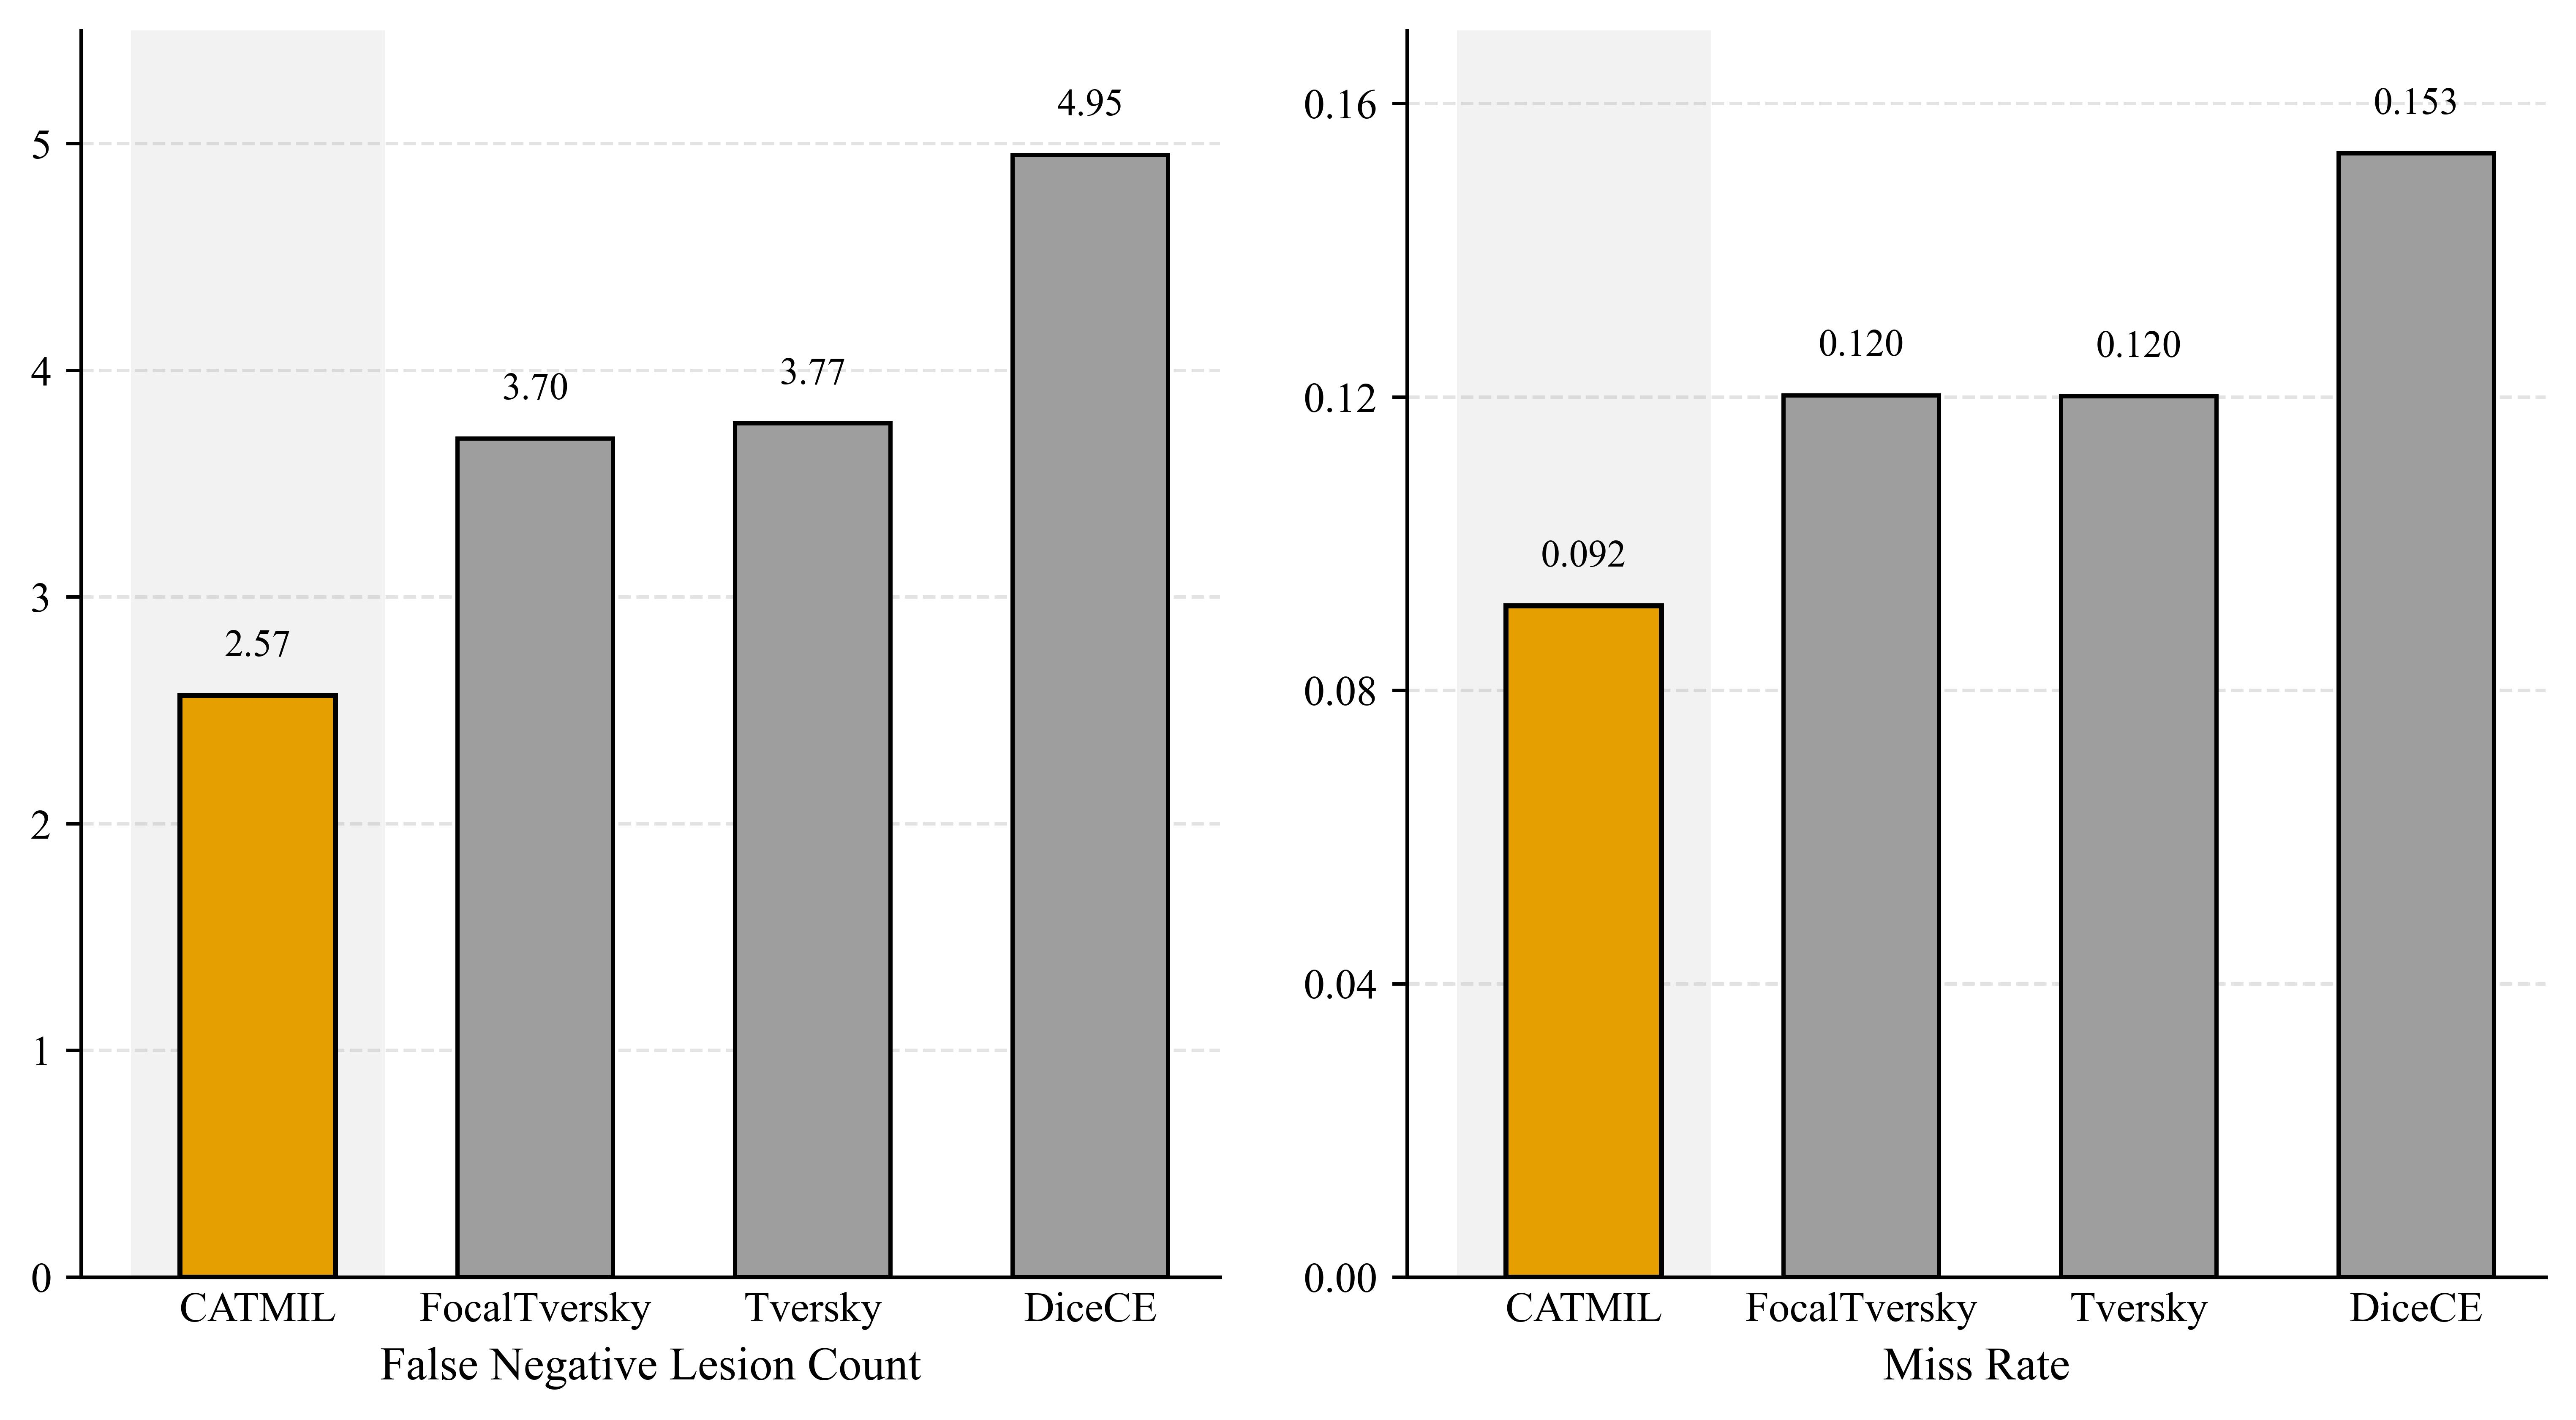
\includegraphics[width=\textwidth]{figures/fn_step1_combined.jpeg}
    \caption{Baseline false negative (FN) analysis across models using lesion-level metrics. From left to right: FN lesion count, lesion recall, and miss rate. nnUNet-CATMIL is highlighted with diagonal stripes.}
    \label{fig:fn_baseline}
\end{figure}

The global FN analysis shows that nnUNet-CATMIL misses fewer lesions
overall, but it does not specify whether the improvement is concentrated
in a particular lesion-size range. We therefore evaluate lesion recall
across size groups in Figure~\ref{fig:fn_recall_by_size}.

nnUNet-CATMIL achieves the highest recall across all lesion-size groups.
The largest relative improvement appears for the smallest lesions
($\leq$10 voxels), where recall increases from 0.14 with nnUNet-DiceCE to
0.33 with nnUNet-CATMIL. This indicates that many tiny lesions that are
completely missed by the standard DiceCE objective can be recovered by the
proposed loss.

The improvement also extends to larger but still small lesions. For
lesions $\leq$50 voxels, nnUNet-CATMIL reaches a recall of 0.79, compared
with 0.71 for nnUNet-DiceCE. For medium-sized lesions ($\leq$200 voxels),
nnUNet-CATMIL achieves 0.95 recall, again outperforming the baselines.
For large lesions ($>200$ voxels), where all methods already perform
well, nnUNet-CATMIL reaches a recall of 1.00. Therefore, the proposed
loss improves detection of the most difficult small lesions without
reducing performance on larger lesions.

These findings suggest that nnUNet-CATMIL reduces the size-dependent bias
commonly observed in lesion segmentation. Standard losses tend to favor
larger and easier structures, whereas CATMIL improves the low-volume
lesion regime while preserving detection of larger components. This
produces a more balanced lesion detection profile across scales.

\begin{figure}[htbp]
    \centering
    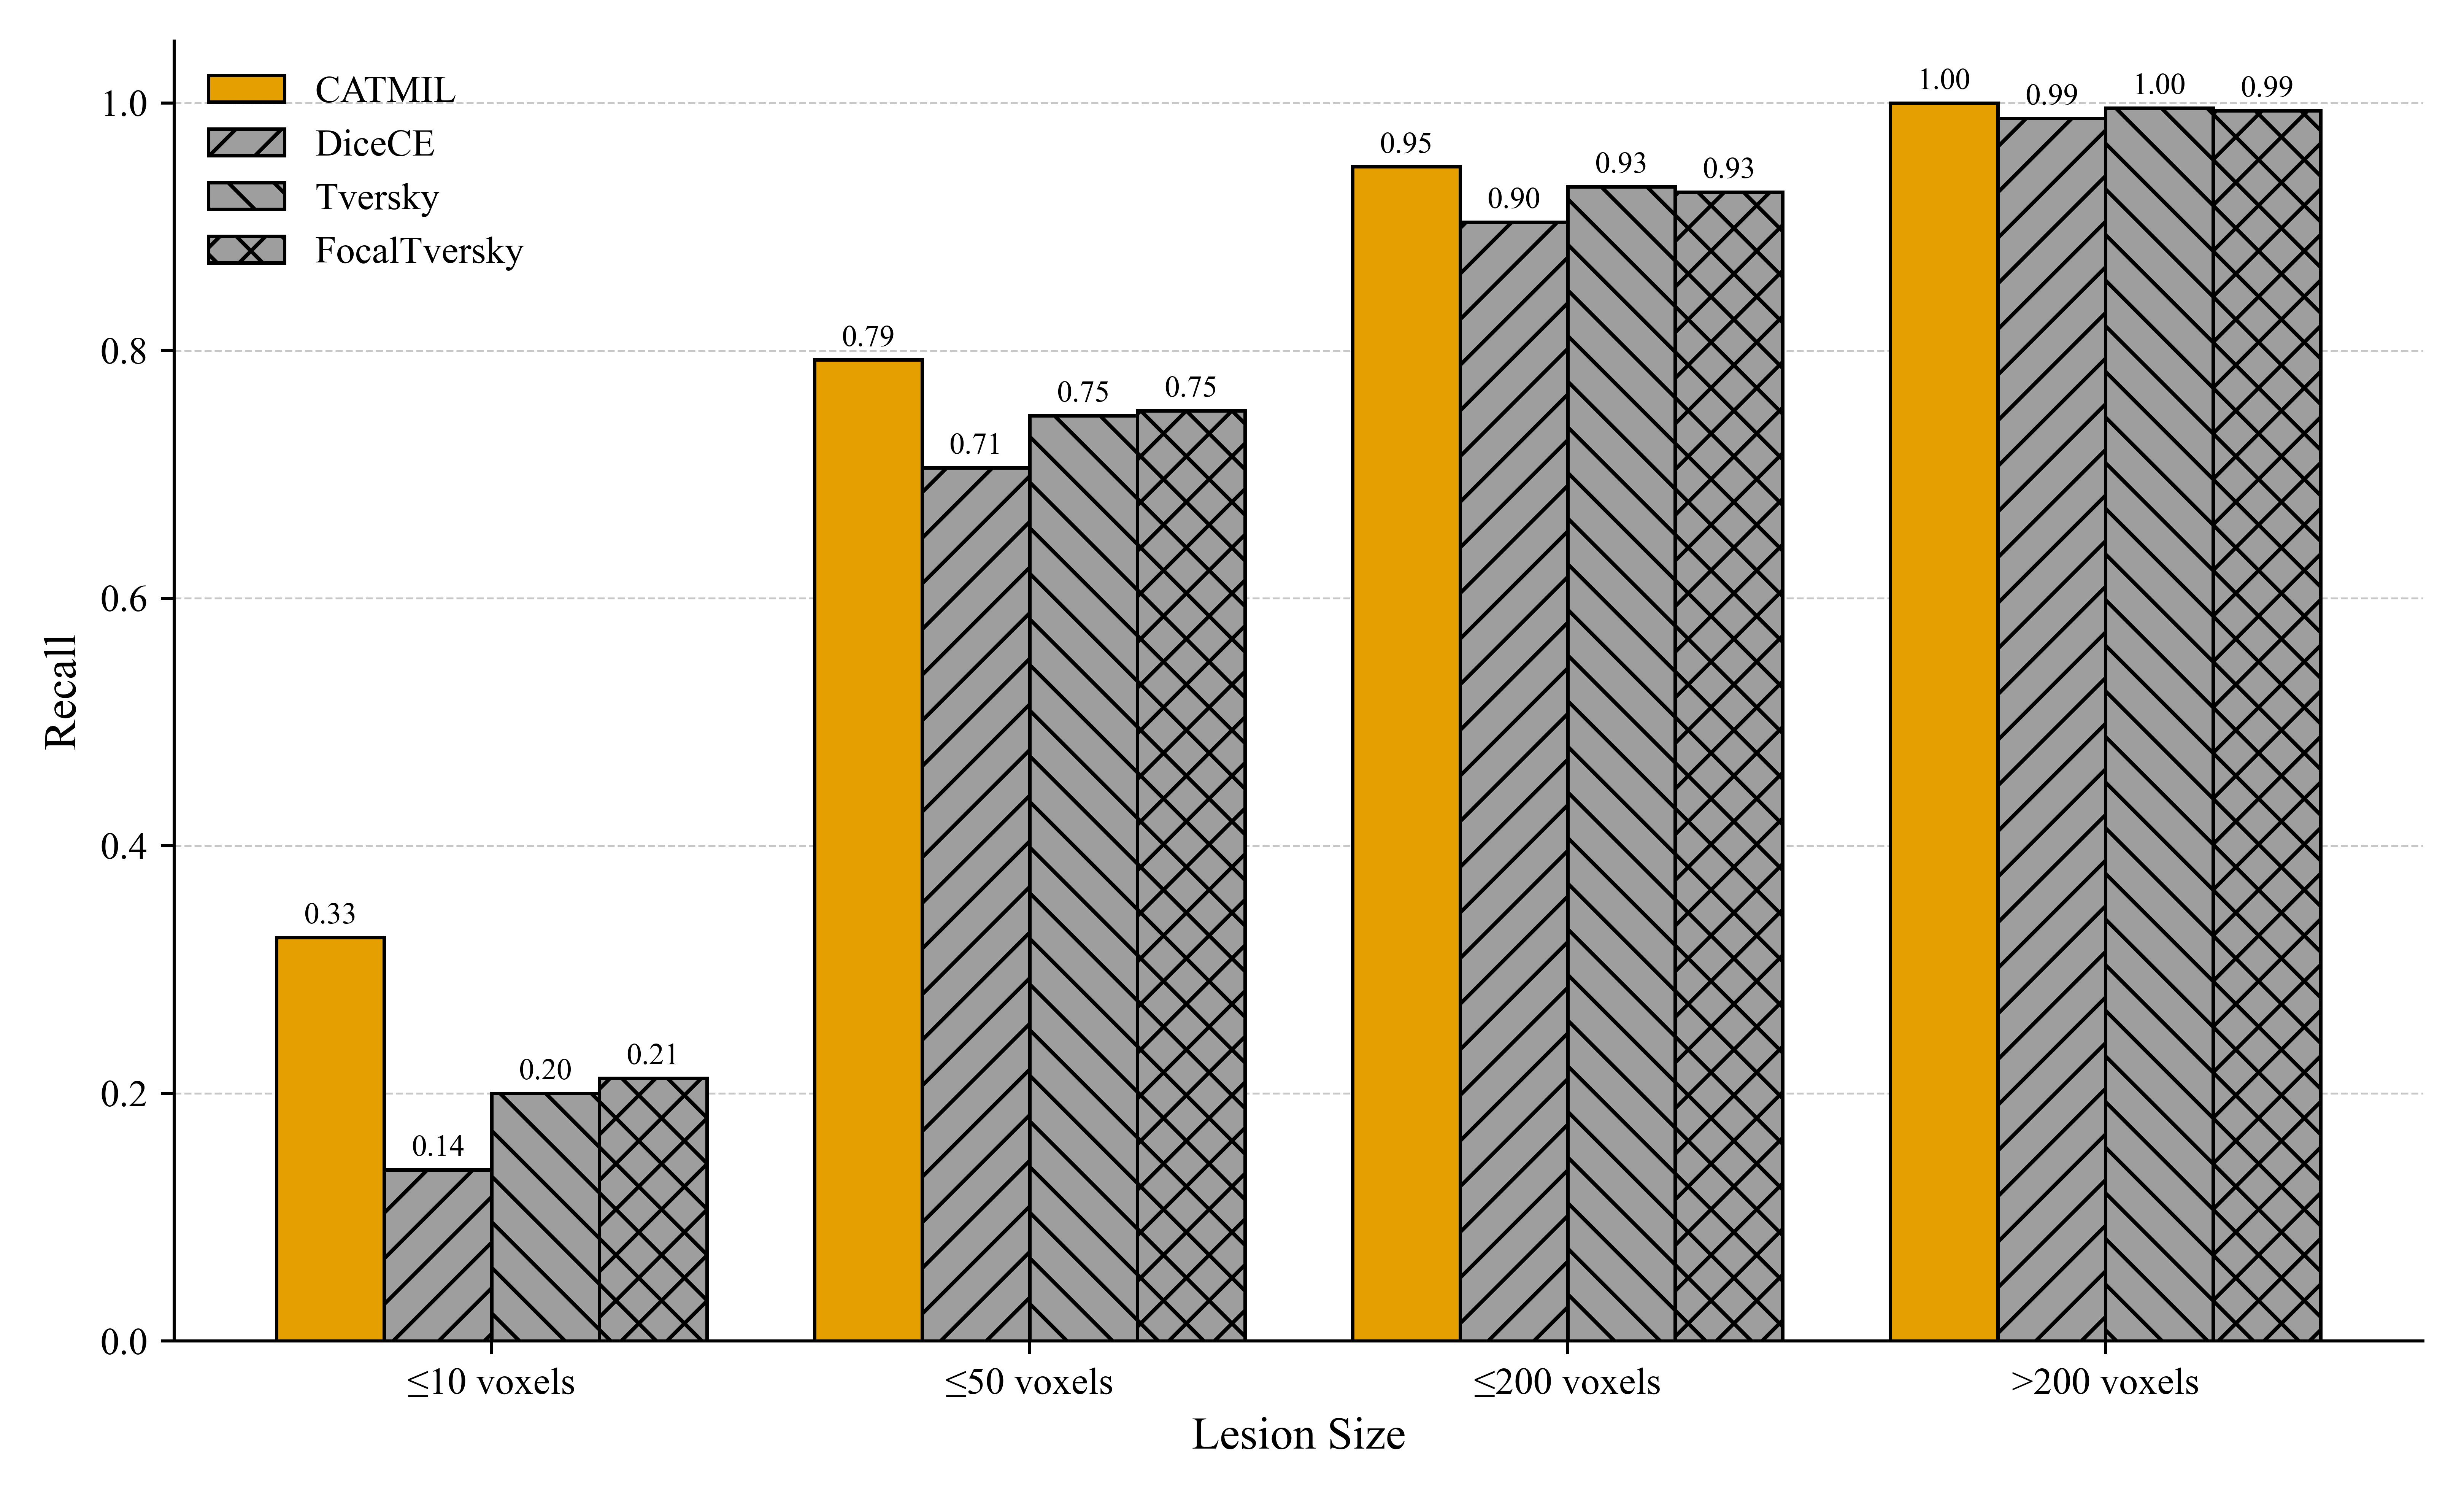
\includegraphics[width=\textwidth]{figures/fn_recall_by_size.jpeg}
    \caption{Recall by lesion size in voxels for different loss functions. Higher recall indicates fewer false negatives.}
    \label{fig:fn_recall_by_size}
\end{figure}


\subsection{Case-Based Qualitative Analysis of Lesion Segmentation}

\begin{figure}[t]
    \centering
    \includegraphics[width=\linewidth]{figures/P47_T1_fold1_slice94_segmentation_comparison.jpeg}
    \caption{
    Segmentation comparison for Case P47\_T1.
    Green indicates correctly detected lesion voxels, red indicates missed
    regions (false negatives), and yellow indicates false positives.
    }
    \label{fig:case_p47}
\end{figure}

Figure~\ref{fig:case_p47} shows Case P47\_T1, where lesions appear in a
clustered pattern with moderate size and relatively visible contrast. The
lesions include components of approximately 20--50 voxels, and their
contrast relative to the surrounding tissue is sufficiently high
(LCNR $>$ 1.5) to make them detectable, although their limited size still
poses a segmentation challenge. All models detect the larger components,
but nnUNet-DiceCE and nnUNet-Tversky miss several smaller regions.
nnUNet-CATMIL detects more of these small components and produces a more
spatially consistent prediction. The segmented regions also align more
closely with the ground truth, suggesting improved handling of clustered
small-lesion structures.

\begin{figure}[t]
    \centering
    \includegraphics[width=\linewidth]{figures/P49_T2_fold1_slice90_segmentation_comparison.jpeg}
    \caption{
    Segmentation comparison for Case P49\_T2.
    Green indicates correctly detected lesion voxels, red indicates missed
    regions (false negatives), and yellow indicates false positives.
    }
    \label{fig:case_p49}
\end{figure}

Case P49\_T2, shown in Figure~\ref{fig:case_p49}, contains elongated
lesions with heterogeneous intensity and less distinct boundaries. The
lesion contrast is relatively low (LCNR $\sim$0.8--1.2), and the weaker
boundary sharpness makes localization more ambiguous. Under this setting,
baseline losses show several missed regions, particularly for small and
low-contrast components, and they also introduce scattered false-positive
areas. nnUNet-FocalTversky improves lesion recovery but produces
irregular segmentation boundaries. nnUNet-CATMIL provides a more balanced
prediction by detecting a larger portion of the difficult lesions while
maintaining more coherent segmentation regions. Although some small false
positives remain, they are limited and do not dominate the predicted mask.

\begin{figure}[t]
    \centering
    \includegraphics[width=\linewidth]{figures/P52_T2_fold0_slice87_segmentation_comparison.jpeg}
    \caption{
    Segmentation comparison for Case P52\_T2.
    Green indicates correctly detected lesion voxels, red indicates missed
    regions (false negatives), and yellow indicates false positives.
    }
    \label{fig:case_p52}
\end{figure}

Figure~\ref{fig:case_p52} presents Case P52\_T2, which represents a highly
sparse lesion scenario. The lesions are very small, with volumes below
approximately 10 voxels, and their contrast is close to the background
noise level (LCNR $\approx$1.0). Such cases are sensitive to minor
prediction errors because the target structures occupy only a few voxels.
Most models detect the main lesion regions, but nnUNet-CATMIL also
produces a small isolated false-positive blob. This example illustrates
the sensitivity-oriented behavior of CATMIL: the model is less likely to
miss weak lesion signals, but this can occasionally introduce small
spurious components in extremely sparse cases. Nevertheless, the main
lesion locations remain correctly identified.

Across the three cases, lesion difficulty is determined by more than
volume alone. Low contrast, weak boundaries, elongated shapes, and sparse
spatial distribution all increase the risk of missed detections. The
qualitative results are consistent with the quantitative findings:
nnUNet-CATMIL improves recovery of subtle lesions and preserves coherent
lesion structures, while the additional false positives are generally
small and localized.


\subsection{Analysis of False Positives and Post-Processing}

The results in Table~\ref{tab:loss_comparison_small_lesion} show an
apparent trade-off in nnUNet-CATMIL. The model achieves the best Dice,
HD95, Small Lesion Recall, FN Count, FN Volume Fraction, and FP Volume,
but its Lesion F1 is lower than the baselines. To interpret this behavior,
we further examine the nature of its false positives.

nnUNet-CATMIL reaches high lesion-level recall, but its lesion-level
precision is lower. This means that the model detects most true lesions,
but it also predicts additional connected components. However, the low FP
Volume indicates that these additional components are not large
over-segmented regions. Instead, the model predicts many small components:
the average number of predicted connected components is much higher than
the number of ground-truth lesions, while the total false-positive volume
remains the lowest among all methods. This suggests that the lower Lesion
F1 is mainly caused by small fragmented predictions rather than extensive
false-positive regions.

The spatial distribution of false positives supports this interpretation.
Most false-positive voxels are located close to ground-truth lesions, with
a near-voxel fraction of approximately 0.7--0.8 and a median distance of
only 1--2 mm. Therefore, many false positives correspond to small
near-lesion fragments or boundary-adjacent predictions, rather than
distant isolated errors. This error pattern is consistent with a model
that is more sensitive to weak lesion evidence.

Since many of these components are small, we apply a simple
post-processing step that removes connected components smaller than
5 voxels. The same procedure is applied to all models, and the resulting
metrics are reported in
Table~\ref{tab:loss_comparison_small_lesion_pp5}.

\begin{center}
\captionof{table}{Comparison of models after post-processing with minimum connected-component size of 5 voxels.}
\label{tab:loss_comparison_small_lesion_pp5}
\resizebox{\textwidth}{!}{%
\begin{tabular}{lcccc}
\toprule
\textbf{Metric} & \textbf{nnUNet-CATMIL (ours)} & \textbf{nnUNet-DiceCE} & \textbf{nnUNet-Tversky} & \textbf{nnUNet-FocalTversky} \\
\midrule
Dice $\uparrow$ 
& \textbf{0.7842} & 0.7797 & 0.7707 & \underline{0.7803} \\

HD95 (mm) $\downarrow$ 
& \textbf{8.1028} & 9.0895 & 10.3585 & \underline{8.2297} \\

Small Lesion Recall $\uparrow$ 
& \textbf{0.8554} & 0.7853 & \underline{0.8223} & 0.8196 \\

Lesion F1 $\uparrow$ 
& 0.8415 & \textbf{0.8586} & 0.8532 & \underline{0.8582} \\

FN Count $\downarrow$ 
& \textbf{3.1333} & 5.2333 & \underline{4.0667} & 4.0833 \\

FN Volume Fraction $\downarrow$ 
& \textbf{0.0238} & 0.0353 & 0.0277 & \underline{0.0270} \\

FP Volume (mm$^3$) $\downarrow$ 
& \textbf{1515} & \underline{1815} & 2618 & 2279 \\
\bottomrule
\end{tabular}%
}
\end{center}

Post-processing produces a similar effect across all losses. Removing
very small connected components slightly reduces recall-related metrics
and increases FN-related metrics, while improving Lesion F1. This
expected trend confirms that the filtering step removes small predicted
regions, some of which correspond to false positives and some of which may
overlap with true small lesions.

For nnUNet-CATMIL, the effect is particularly informative. Lesion F1
increases substantially from 0.7571 before post-processing to 0.8415
after filtering, showing that many of the lesion-level precision errors
come from very small components. At the same time, nnUNet-CATMIL retains
the best Dice score, the lowest HD95, the highest Small Lesion Recall,
the lowest FN Count, the lowest FN Volume Fraction, and the lowest FP
Volume after post-processing. Therefore, the post-processed results
preserve the main advantage of CATMIL while reducing the lesion-level
precision penalty.

Overall, these results indicate that nnUNet-CATMIL favors sensitivity to
small and weak lesion signals. This sensitivity can introduce additional
small connected components, but these components are limited in volume and
can be reduced by a simple model-agnostic post-processing step. After
filtering, CATMIL continues to show the strongest overall balance between
segmentation quality, missed-lesion reduction, and false-positive control.

\section{Conclusion \& Discussion}
This study shows that modifying the training objective is an effective way
to control model behavior in sparse lesion segmentation. Rather than
increasing architectural complexity, the proposed approach redistributes
supervision during optimization, enabling clearer interpretation of its
effects. Voxel-wise objectives inherently favor high-volume regions, causing small
lesions to have limited influence. The proposed objective addresses this
through two terms: a component-adaptive term that balances contributions
across lesion structures, and a lesion-level term that enforces lesion
detection. Together, these shift learning from purely overlap-driven
optimization toward better sensitivity to sparse lesion signals. Results support this design. The method improves small lesion recall and reduces false negatives while maintaining competitive Dice and improving
boundary accuracy, indicating balanced performance across metrics. However, increased sensitivity leads to reduced lesion-wise precision, often due to small isolated false positives or fragmented predictions.
This reflects a trade-off between detection and delineation, further
affected by the lesion-level term, which enforces detection but not full
coverage. Lesion detectability also depends on factors such as contrast and boundary
clarity. While the proposed objective improves sensitivity, it does not
fully overcome limitations in input data. Limitations include evaluation on a single dataset, focus on one disease,
and use of a single architecture. In addition, the detection–precision
trade-off is not explicitly controlled. Future work should evaluate generalization across datasets and diseases,
validate across architectures, and improve control over false positives
and boundary consistency. Extending lesion-level supervision to include
coverage constraints may further improve segmentation quality. Overall, the results suggest that small lesion segmentation depends on how sparse signals are represented during learning. The proposed objective
improves sensitivity to small lesions while maintaining stable global
performance, highlighting the role of loss design in imbalanced settings.

\paragraph{Acknowledgements.}
This work was supported by a grant for research centers, provided by the Ministry of Economic Development of the Russian Federation in accordance with the subsidy agreement with the Novosibirsk State University dated April 17, 2025 No. 139-15-2025-006: IGK 000000C313925P3S0002

\bibliographystyle{unsrtnat}
\bibliography{references}

\newpage
\section*{Ablation}
To better understand the contribution of each component in the proposed
objective, we conduct two controlled ablation experiments under the same
training and evaluation protocol.

\paragraph{Experimental Setup.}
All ablation experiments are performed using the same \texttt{nnUNet}
configuration, data splits, preprocessing, and training schedule as in
the main experiments. All models are evaluated using voxel-level and lesion-level metrics,
including Dice, HD95, lesion-wise F1, small lesion recall, and false
positive characteristics, to provide a comprehensive assessment of model
behavior in the sparse lesion regime.

\subsection*{Ablation I: Contribution of CAT and MIL Terms}

To isolate the effect of each component, we compare three variants:
(i) nnUNet-CAT, which incorporates only the structure-level
component-adaptive term,
(ii) nnUNet-MIL, which incorporates only the lesion-level supervision
term, and
(iii) nnUNet-CATMIL, which combines both terms into a unified objective.

Table~\ref{tab:ablation_cat_mil} reports the mean performance across
5-fold cross-validation. The results reveal a clear trade-off between the
two terms. nnUNet-CAT achieves the highest lesion-wise F1 (0.8386) but
lower small lesion recall (0.8230), indicating stronger structural
consistency but limited sensitivity to small lesions. In contrast,
nnUNet-MIL improves small lesion recall (0.8712) but degrades boundary
accuracy (HD95 = 9.2375 mm) and lesion-wise F1 (0.7492), reflecting less
precise segmentation. The combined nnUNet-CATMIL achieves the most balanced performance. It
obtains the best Dice (0.7834) and lowest HD95 (7.9817 mm), while also
achieving the highest small lesion recall (0.8730) and the lowest FP blob
fraction (0.2094). This indicates that combining CAT and MIL mitigates
their individual limitations, improving both detection of small lesions
and overall segmentation quality without increasing false positives.

\begin{table}[H]
\centering
\caption{Ablation study on the contribution of CAT and MIL terms.}
\label{tab:ablation_cat_mil}
\begin{tabular}{lcccccc}
\hline
Model & Dice & HD95 $\downarrow$ & Lesion F1 & Small Lesion Recall & FP Vol & FP Blob \\
\hline
nnUNet-CAT    & 0.7812 & 8.6844 & 0.8386 & 0.8230 & 1528.72 & 0.2277 \\
nnUNet-MIL    & 0.7805 & 9.2375 & 0.7492 & 0.8712 & 1539.77 & 0.2195 \\
nnUNet-CATMIL & \textbf{0.7834} & \textbf{7.9817} & 0.7571 & \textbf{0.8730} & 1536.88 & \textbf{0.2094} \\
\hline
\end{tabular}
\end{table}

\subsection*{Ablation II: Sensitivity to Loss Weights}

We analyze the impact of different weighting coefficients
$\lambda_{\text{CAT}}$ and $\lambda_{\text{MIL}}$ on model performance.
The results in Table~\ref{tab:ablation_lambda} reveal a clear trade-off
between segmentation accuracy and lesion-level detection.

\begin{table}[H]
\centering
\caption{Sensitivity analysis of $\lambda_{\text{CAT}}$ and $\lambda_{\text{MIL}}$.}
\label{tab:ablation_lambda}
\begin{tabular}{lccccc}
\hline
Model & Dice & HD95 $\downarrow$ & Lesion F1 & Small Recall & FP Vol $\downarrow$ \\
\hline
CATMIL0101 & 0.7675 & 9.3881 & 0.7720 & 0.8514 & 2292.17 \\
CATMIL0102 & \textbf{0.7954} & \textbf{5.9771} & 0.7452 & 0.8711 & 1345.83 \\
CATMIL0201 & \underline{0.7921} & \underline{6.7964} & \textbf{0.7754} & \textbf{0.8784} & \textbf{1233.92} \\
CATMIL0202 & 0.7663 & 9.4507 & 0.7632 & \underline{0.8699} & \underline{1729.42} \\
\hline
\end{tabular}
\end{table}

Lower weights (CATMIL0102) lead to the best global segmentation
performance, achieving the highest Dice (0.7954) and lowest HD95
(5.9771 mm), indicating improved overlap and boundary accuracy. However,
this comes with reduced lesion-wise F1 (0.7452), suggesting weaker
instance-level consistency. In contrast, higher weights (CATMIL0201) improve lesion-level behavior,
achieving the highest lesion F1 (0.7754), highest small lesion recall
(0.8784), and lowest FP volume (1233.92 mm$^3$). This indicates stronger
detection of small and sparse lesions with better control of false
positives, albeit with slightly reduced Dice and boundary accuracy. These results confirm that $\lambda_{\text{CAT}}$ and
$\lambda_{\text{MIL}}$ control the balance between voxel-level accuracy
and lesion-level sensitivity. Moderate weighting provides a balanced
solution, while higher weights emphasize detection and lower weights
favor precise segmentation.

\end{document}